\chapter{Experimental Setup}
\section{Synchrotron Radiation}
The radiation emitted by a relativistic charged particle, usually electrons, accelerated to a circular orbit through an external magnetic field is called synchrotron radiation. This radiation is polarized and emitted tangential to the circular movement of the charged particle in forward direction. In the history of synchrotron radiation sources have evolved from parasitic use at particle accelerators to the extend of building electron storage rings dedicated for the sole purpose of generating this radiation \cite{munro_chapter_1987}. Its most promitent features are the high brilliance, that is the number of photons per second per unit particle beam cross section and per unit solid angle within $0.1\%$ bandwidth at a specific wavelength, and its huge spectral range of emission. Depending on the energy of the relativistic particles forced on a circular orbit, in modern electron storage rings typically in the order of one to several GeV, the emission covers the range from the terahertz into the hard X-ray regime. The \gls{ptb} operates two laboratories at the dedicated sources \gls{bessy} and the \gls{mls} \cite{brandt_metrology_2007}. The two thrid-generation synchrotron radiation sources provide maximum electron energies of $1.7$ GeV (\gls{bessy}) and $0.6$ GeV (\gls{mls}), respectively. Theoretical emission spectra are shown in Fig.~\ref{ch_exp:fig_experimental_synchrotron_spectra} in comparison to black body radiation.
\begin{figure}
 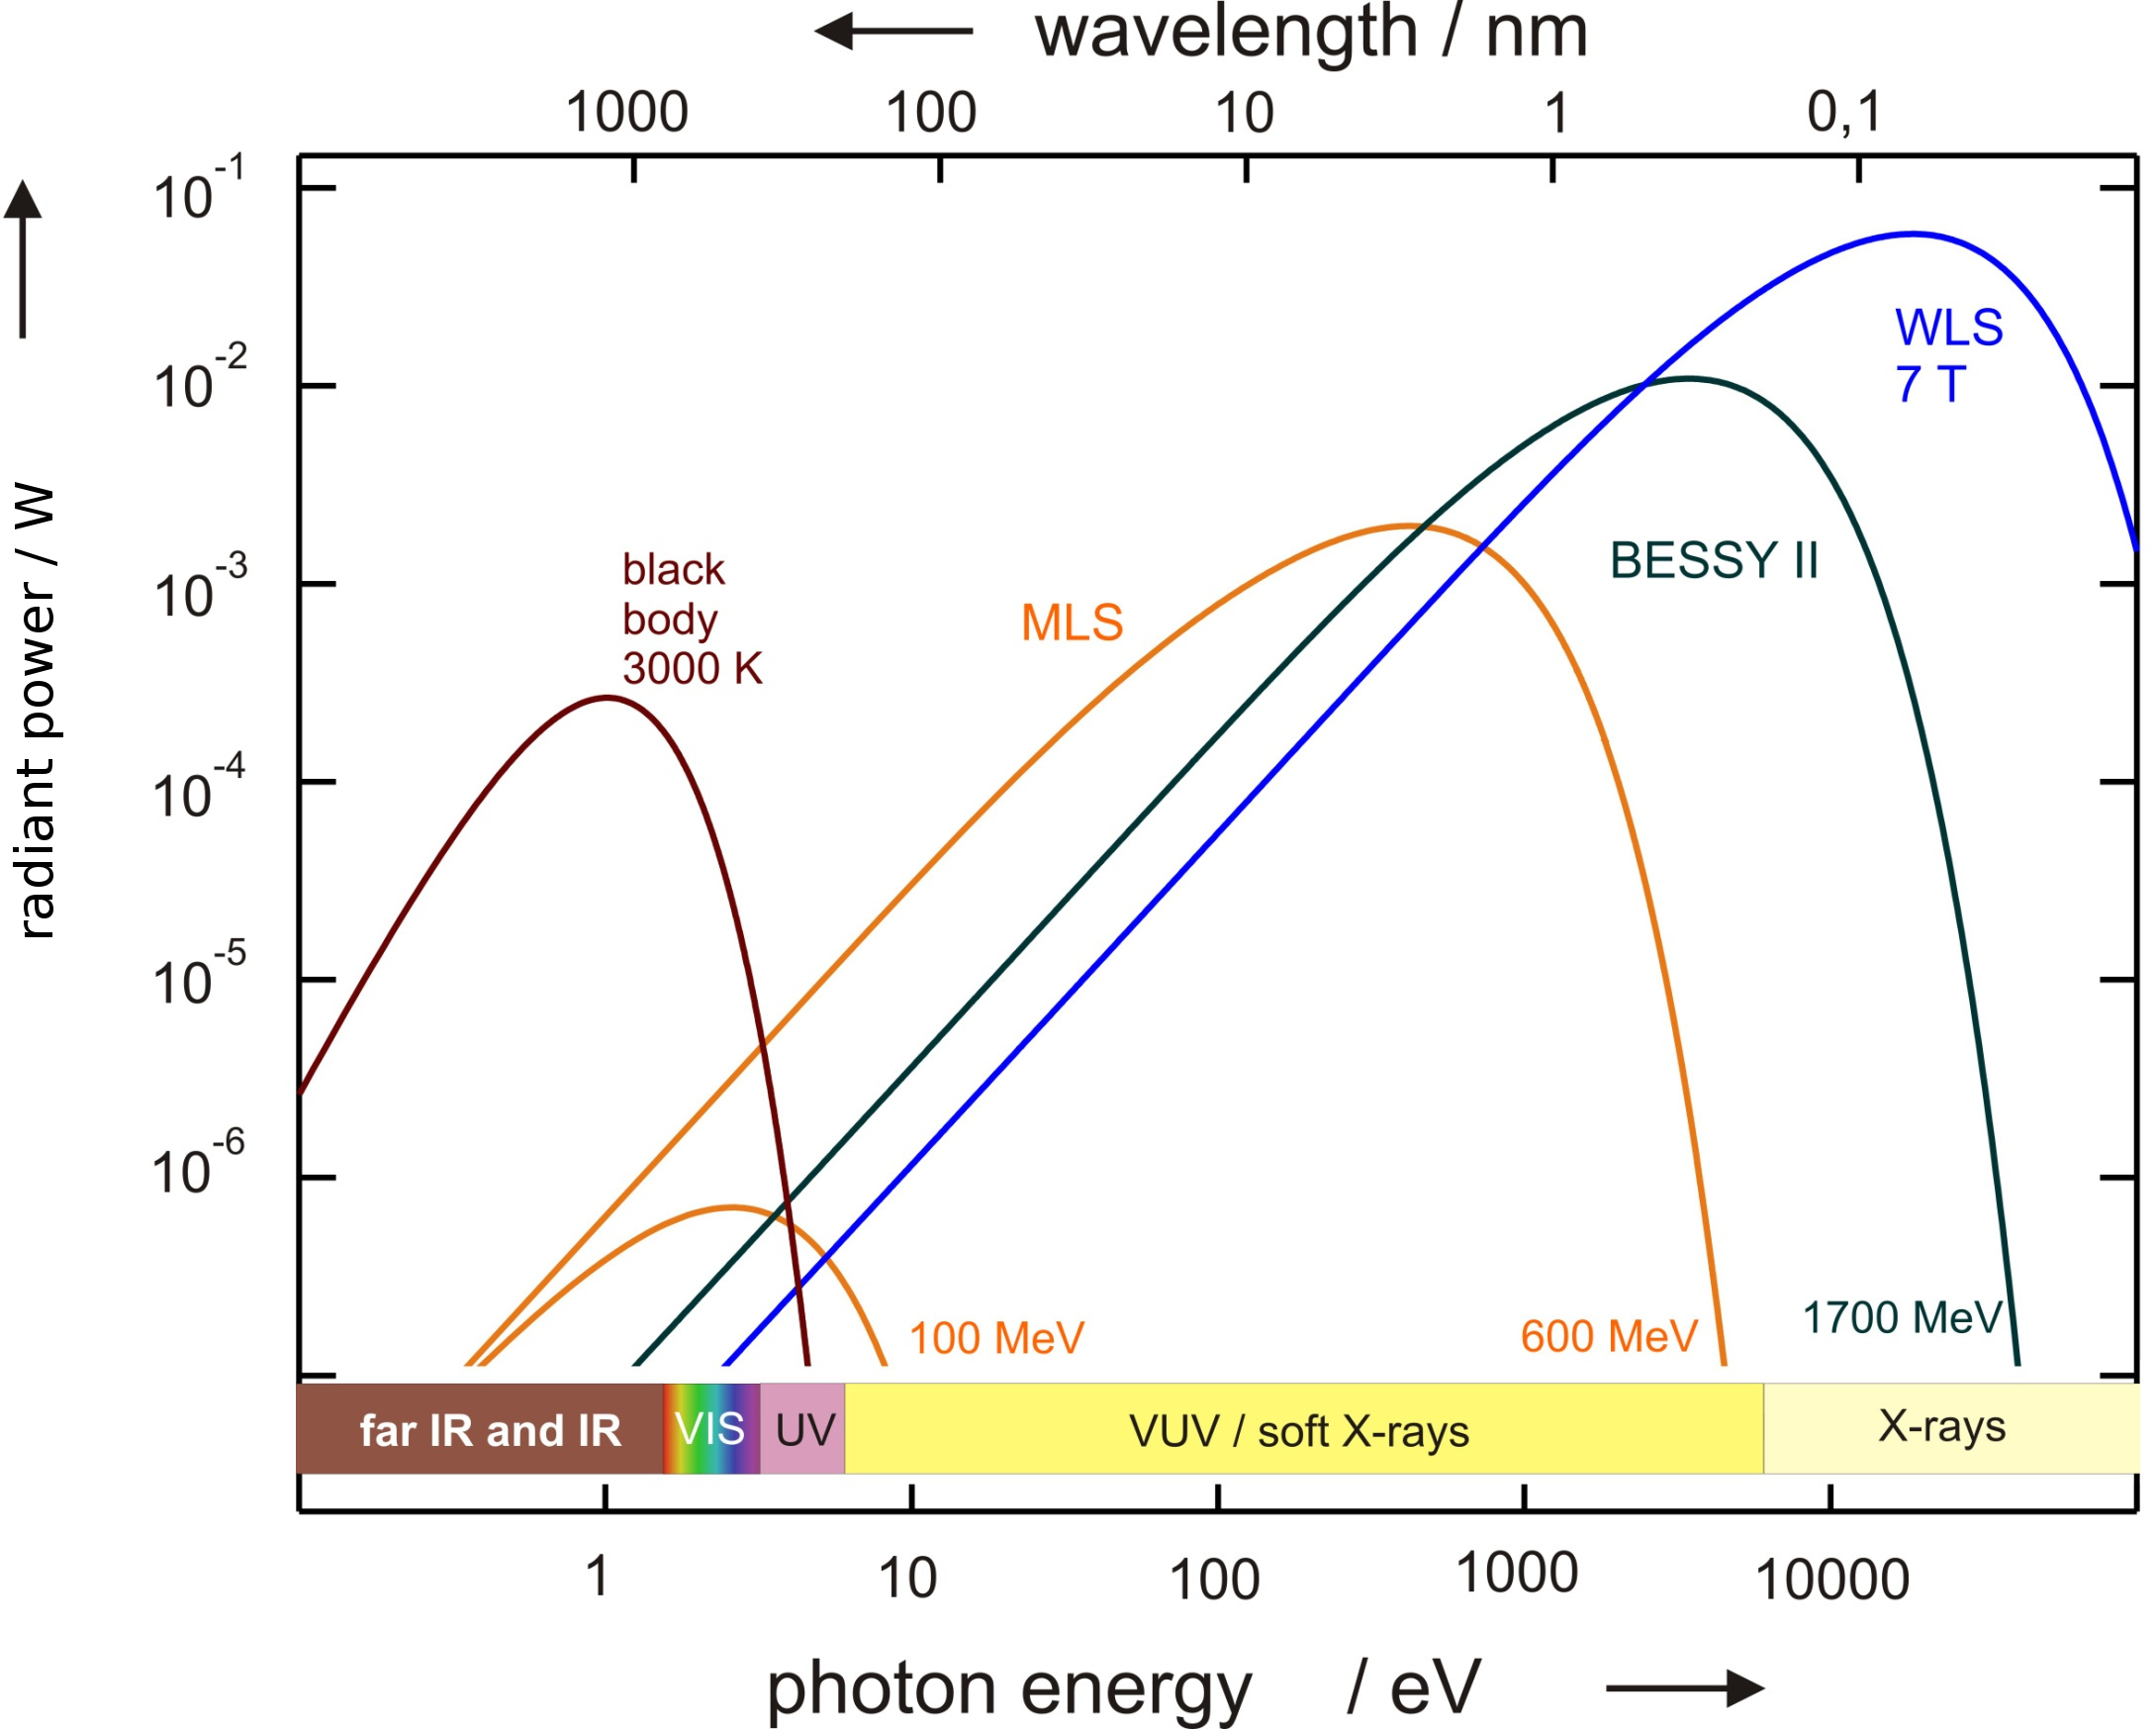
\includegraphics[width=0.7\textwidth]{img/exp-bessy-dipole-spectrum.jpeg}
 \caption[Theoretical synchrotron radiation radiant power spectra]{Theoretical synchrotron radiation radiant power spectra for the \gls{mls} and \gls{bessy} in comparison to black body radiation\footnote{Image taken from Beckhoff et al.~\cite{beckhoff_quarter-century_2009}}. The curves show the radiant power of emission for bending magnets at both electron storage ring facilities for different electron energies. The curve marked WLS shows the radiant power from the $7$ Tesla wavelength shifter insertion device installed at \gls{bessy}.}
 \label{ch_exp:fig_experimental_synchrotron_spectra}
\end{figure}

A very important theoretical aspect of synchrotron radiation, apart from the high brilliance and large spectrum, is the fact that the emission can be calculated exactly from first principles of classical electrodynamics. The theory specific for synchrotron radiation was developed by Schwinger \cite{schwinger_classical_1949} and we shall review its most imporant aspects here. Given all the fundamental and experimental parameters are known, the emitted radiant power per relativistic particle can be calculated exactly as
\begin{align}
 P = \frac{1}{4 \pi \gls{epsilon_0}} \frac{2}{3} \frac{\gls{e}^2 \gls{c}}{R^2}\Big( \frac{E}{\gls{m_0} \gls{c}^2}\Big)^4 \text{,} \label{ch_exp:schwinger_equation}
\end{align}
where \gls{e} is the elementary charge, \gls{c} is the speed of light in vacuum, $E$ is the particles energy, \gls{m_0} is the rest mass of the particle and $R$ is the radius of the circular trajectory imposed by the magnetic field. The radiant power is thus inversely proportional to the fourth power of the particles rest mass, which explains the usage of light electrons in comparison with significanlty heavier protons in synchrotron radiation sources. The dependence on the electron energy is visible in another characteristic value for the emitted radiant power, visible as a shift to higher photon energies (smaller wavelengths) in Fig.~\ref{ch_exp:fig_experimental_synchrotron_spectra}, known as the critical energy or critical wavelength \cite{schwinger_classical_1949}, respectively,
\begin{align}
 E_C = \frac{3 \gls{h} \gls{c}}{4 \pi R} \Big( \frac{E}{\gls{m_0} \gls{c}^2}\Big)^3 \text{.} \label{ch_exp:characteristic_energy}
\end{align}
It marks the point in the spectrum, where the integrated radiant power for all values above and below the critical energy are equal. This formula quantifies the shift towards higher energies due to the increase of the electron energy comparing the \gls{mls} and \gls{bessy} emission spectra.

The ability to calculate the exact emission properties of synchrotron radiation have another very valuable side effect for the purpose of metrology. It enables the use of synchrotron radiation as a primary standard for electromagnetic radiation, which is in fact exploited by the \gls{ptb} \cite{thornagel_electron_2001}.



\section{The SX700 and EUVR Beamlines}
\begin{figure*}[htb]
    \def\svgwidth{\textwidth}
    \import{svg/}{exp-ptb-beamlines.pdf_tex}
    \caption[PTB Beamlines in the BESSY II laboratory.]{Beamlines in the laboratory at \gls{bessy}.}
    \label{ch_exp:fig_beamlines_bessy}
\end{figure*}
SX700 \cite{beckhoff_quarter-century_2009}
\section{The ELLI and BigRef Reflectometers}
BigRef \cite{scholze_high-accuracy_2001}
ELLI \cite{soltwisch_polarization_2015}
\section{Grazing-incidence X-ray Fluorescence at the FCM Beamline}